\chapter{Methodology}
\label{example}
%In diesem Kapitel beschreiben Sie Ihren eigenen Beitrag
%- Es muss klar sein, worin die eigentliche Innovation besteht#

\section{Research Questions}
For this thesis we have selected 3 research questions. The first question : Can we use the visualization techniques to identify relevant properties of one performance-Influence model? The performance-influence models are of the format mentioned below:

\begin{equation*}
  \pi {(c)} = \overbrace{\underbrace {3}_{Coeff.} \cdot  \underbrace{{c(A)}}_{Option}}^{Term 1}  + \overbrace{ \underbrace{5}_{Coeff.} \cdot \underbrace{{c(B)}}_{Option}}^{Term 2} + \overbrace{\underbrace{0}_{Coeff.} \cdot \underbrace{{c(C)}}_{Option}}^{Term 3} - \overbrace{\underbrace{4}_{Coeff.} \cdot \underbrace{{ c(A)} \cdot {c(B)}}_{Interaction}}^{Term 4}
\end{equation*}

The set of valid performance-influence models are put into a csv file. And these csv files are used as an input for the visualization. 

From the visualizations we can identify the data point that is either the highest or lowest point that influences the systems performance the most.

Second research question : Can we use the visualization to compare two performance-influence models?. Many times a version of a software needs to be compared to its next version to check how the two versions differ in terms of its performance. In this case, we have two performance-influence models in one csv file, and use this as an input to the visualization. hence comparison of two different performance-influence models can be done, and identify if the same configuration option causes a spike in performance in either of the versions.

Third research question : How do the visualizations scale?. when a configurable software has added new configuration options, new performance-influence models are derived to reflect its performance influence over the system. The new performance-influence models are then used as an input to the visualization. Scaling can be of two types. One, addition of new configuration option. Two, addition of new performance-influence model to the same csv file. Both of the types of scaling are implemented in the thesis.

\section{Why the above Research Questions?}
The research questions are selected based on number of performance-influence models we visualize at the same time. When we have only one performance-influence model, we would like to know the configuration option that has affected the performance the highest, it can be maximum performance increase or decrease. 

when we look at the two performance-influence models, we are basically comparing the two and finding out the configuration that either differs the most or is the most similar. The configuration option that differs the most can indicate that this configuration option has caused a performance spike in one of the versions, it can be positive or negative spike. The configuration option that have been the most similar indicate that in the second version of the software, this configuration option remained unaffected.

when we look at more than 2 performance-influence models, we have comparing several versions of the same software with increasing configuration options in each versions. This visualization helps to see what would be the outliers, or which set of performance-influence models have share similar set of influences.

\section{How do we plan on getting the answers to these questions?}

we use three different visualization tecnhiques to help us answers the research questions. Each visualization has its own steps to get to the answers.

Question 1: The  most relevant configuration option or interaction would be the one which makes highest positive or most negative effect. The configuration option or interaction which makes zero effect would be also of interest here.

 Radar Chart:  For this visualization, we identify the data point that is plotted far most in the outer circle which indicates that it makes the most negative effect on performance, or the data point that is plotted closer most to the inner circle which indicates that it makes the most postive effect on performance. If there are two data points that are very close to each other, we can use the tooltip to see the exact value that it contributes. Hence we can come to a conclusion on one single data point that would make the most postive or the most negative effect on performance of the entire system. For the configuration option or interaction which makes zero effect, we need to identify the data point which is plotted with a white round symbol.

 Text Plot : For this visualization, we identify the data point that is closest to either of the border lines of the plot. The data point which is closest to the left border line indicates that it makes the most positive effect on the performance. whereas the data point which is closest to the right border line indicates that it makes the most negative effect on the performance. If there are two data points which are very close to each other and are not able to be distinguished, we can use the tooltip to hover over both the data points to look at the exact value that it contributes and hence know the most relevant configuration option or interaction. For the configuration option or interaction that makes zero contriubution towards the performance, we need to identify the data points marked with an inner white marker symbol. These are the configuration options or interactions which makes no contribution towards the performance of the entire system.

 Ratio Plot : For this visualization, we know that the bars are sorted according to the amount of performance it contributes. Hence it is very easy to identify the configuration option or interaction which makes the highest performance affect. It the first bar in the visualization, and the bar which is to the extreme right indicates that it makes the lowest performance affect. But, this conclusion is when we do not consider the sign of the data points. For example, the first bar makes the highest performance affect, but we do not know if it makes most positive or most negative effect on performance, it can be either postive or negative. For that configuration option or interaction that makes zero effect on performance, it is again hard to identify since these configuration options are not plotted in the graph at all.

 Question 2 : Often times a developer or an user would need to compare two versions of the same software to identify if there are any performance spikes or an introduction of a performance bug. In this case, we use the performance-influence models of the two different versions in the same csv files as different groups. The different groups are plotted as two different plots in the same graphs hence the comparision is easier.

we can use the two different plots to identify the configuration option or interaction that are the most similiar to each other, which indicates that the performance contributed by this configuration option or interaction is not affect in the newer version. we can also use the different plot to identify the configuration option or interaction which are most different to each other, which indicates that the performance contributed by this configuration option or interation is affected the most by introduction of the newer version. This can also indicate the introduction of the performance bug.

 Radar Chart: For this visualization, we need to identify the corresponding data point in both the plots which are most closer to each other or most far away from each other. The data points which are most close to each other indicate that  corresponding configuration option or interaction contributes the same/ similar amount of performance to the performance of the entire system. The data points which are most far away from each other indicate  that the corresponding configuration option or interaction has a spike in performance in the newer or older version of the software. It can also indicate that the newer version of the software has introduced a performance bug with respect to the corresponding configuration option or interaction. 


 Text Plot : For this visualization, we need to identify the corresponding data point in both the plots which are most closer to each or the most far away from each other. Both of which make the same conclusion as mentioned above in the radar plot.

 Ratio Plot: For this visualization, we need to identify the bars (configuration option or interaction) which are most similar or same in size and color, which indicates the configuration option or interaction that makes same or similar amount of performance in the newer version of the software as that of the older version. we can also identify the bar that would has the highest difference in the size of the bars but are of the same color. This configuration option or interaction indicates that it contributes to a lot of performance in the newer version than that of the older version. This contribution can be a performance increase or decrease, if its performance increase in the newer version it can also indicate that this configuration option or interaction has introduced a performance bug in the newer version of the software.

 Question 3: Scaling of the visualization techniques can be in two different ways. one, addition of new configuration options or interactions. second, addition of new groups/ plots to the same graph.

Radar Plot and Text Plot: 
Addtion of new configuration option /interaction: Adding new features to configurable softwares indicates that a new configuration option and or an interaction is added to the newly produced performance-influence model. As and when the performance-influence model increases, the size of the visualization also increases in the same order.
Addition of new gorups to the same graph: For comparision of several versions of the software, several groups/ performance-influence models of individual versions are put in the same csv file. Each individual version is mapped as a different plot in the same visualization, which makes comparision of all the versions easier.

Ratio Plot : 
Addtion of new configuration option /interaction: Addition of new configuration option or interaction is added as a new bar in the visualization. As and when the size of the performance-influence model increases, the size of the visualization increases in terms of the number of bars the visualization consists. 
Addition of new gorups to the same graph: For comparision of several versions of the software, several performance-influence models are put in the same csv file and this file is used as an input to the visualization. Each individual version is mapped as a different plot/set of bars in the same visualization, making comparision of several versions at the same time easier.

\section{Interview}

To test the tool and get some feedback, we interviewed possible users of the tool to use it and answer several questions based on the visualization of performance-influence models. The interview consisted of an initial warm--up phase, where the interviwee is given a brief explaination of performance-influence models, configurable software systems, configuration option, interaction etc. The interviewer also explains in brief the working of the tool, so that the interviwee can use the tool themselves to answer the questions.
The questions are separated based on the number of performance-influence models the questions they include. There are three sections, one performance-influence model, two performance-influence models and many performance-influence models. Each section has several questions, each question includes a different performance-influence model for each of the visualization type, namely radar plot, text plot and ratio plot. 
The questions themselves are answered on likert scale indicating how easy or difficult it is for a user to derive the answer the question. If the questions have a definite answer, an area to fill in the answer is provided for the user to enter the answer. Also each question has a comments or feedback area to fill in, if the user has feedback or some input for possible betterment of the visualizations.
Each question is in form of a link, which when clicked opens a new visualization for the user to answer the question.

\section{Questionnaire}
The questionnaire is divided into three sections. Each section having set of questions belonging to either simple performance-influence model or complex performance-influence model.

One performance-influence model
  Question 1: Which is the most relevant configuration option or interaction?
  Question 2: Which is the configuration option or interaction that leads to highest performance increase or decrease?

Two performance-influence models
 Question 1: Which is the configuration option or interaction where the performance-influence models differs the most?
 Question 2: Which is the configuration option or interaction where the performance-influence models are the most similar?

Many performance-influence models
 Question 1: which pair of performance-influence models share a large set of influences?

 Each question has 3 sub sections for three different types of visualizations.

\section{Acronyms}

This template makes advantage of the glossaries package to support acronyms. The first occurence of an acronym is replaced by its definition (e.g., \gls{IDE}). All other occurences are replaced by the acronym (\gls{IDE}). The glossaries package also supports plural---\glspl{IDE}.

\glsreset{IDE}
Sometimes you want to make sure, that the long version is used, even if \gls{IDE} was inserted before.
 
\section{Citation}

There are several types of literature. The most citations are workshop and conference papers. Please use the inproceedings-tag for those citations (e.g., \cite{KAK:GPCE09}). You should have short-hands for workshop and conference names to be sure the naming is consistent and uniform (see our BibTeX files how to do that).
 
Slightly different are articles published in journals (e.g., \cite{KG:SME06}). Make sure you that the volume and number-tags are present and that no inproceeding is tagged as article or vice versa.

You might want to take a look at the example BibTeX file to find out how to cite books~\cite{CE:BOOK00}, technical reports~\cite{KCHNP:TR90}, websites~\cite{Coq:website}, PhD theses, or master theses~\cite{B:PHD03,R:MT09}.

\section{Formulas}
 
There are different types of mathematical environments to set formulas. The equation $E=m\cdot c^2$ is an inline formula. But you can also have formulas at a separate line (see \vref{eq:ex}).

	\begin{equation}\label{eq:ex}
			P=\bigl(\mathcal{A}\pimplies(\mathcal{B}\pequals\mathcal{C})\pand(\mathcal{B}\pequals\mathcal{D})\bigr)\pand(\mathcal{B}\pimplies\mathcal{A})\pand(\mathcal{C}\pimplies\mathcal{A})\pand(\mathcal{D}\pimplies\mathcal{A})
	\end{equation}

If you need multiple lines that are aligned to each other, you might want to use the following code.

	\newcommand{\fG}{\mbox{GraphLibrary}}
	\newcommand{\fE}{\mbox{Edges}}
	\newcommand{\fA}{\mbox{Algorithms}}
	\newcommand{\fD}{\mbox{Directed}}
	\newcommand{\fU}{\mbox{Undirected}}
	\newcommand{\fN}{\mbox{Number}}
	\newcommand{\fC}{\mbox{Cycle}}
	\begin{eqnarray*}
	&& \fG\\
	&\pand& (\fG \pimplies \fE) \pand (\fE \por \fA \pimplies \fG)\\
	&\pand& (\fE \pequals \fD \por \fU) \pand (\pnot \fD \por \pnot \fU)\\
	&\pand& (\fA \pequals \fN \por \fC)\\
	&\pand& (\fC \pimplies \fD).\\
	\end{eqnarray*}

\section{Graphics}

In \vref{fig:ex}, we give a small example how to insert and reference a figure.

\begin{figure}[htbp]
	\centering
		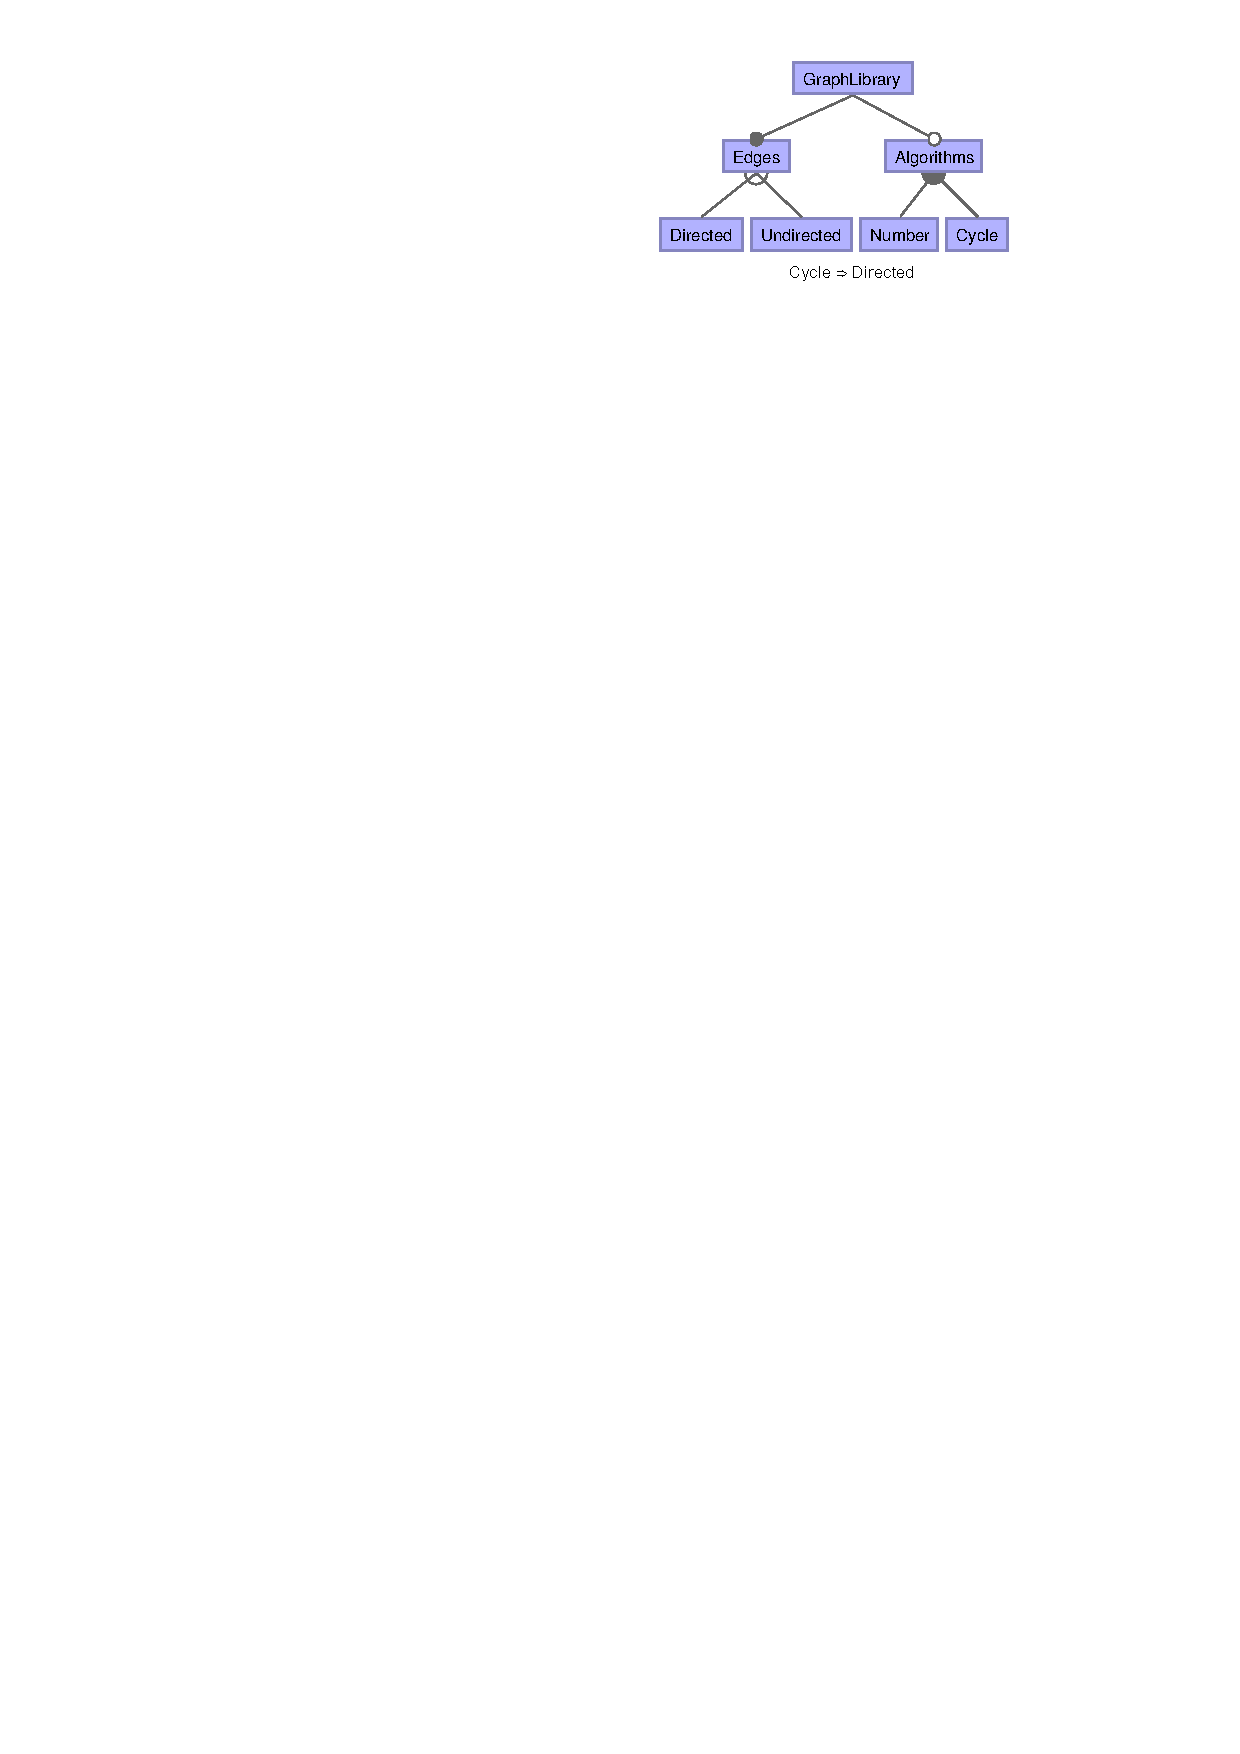
\includegraphics[scale=1.25]{example}
	\caption{A feature model representing a graph product line}
	\label{fig:ex}
\end{figure}

\section{Tables}

\vref{tab:ex} shows the result of a simple tabular environment.

\begin{table}[htbp]
	\centering
		\begin{tabular}{cc}\toprule
			Group Type & Propositional Formula\\\midrule
			And & $(P \pimplies C_{k_1} \wedge\ldots\wedge C_{k_m}) \pand (C_1\vee\ldots\vee C_n \pimplies P)$\\\addlinespace
			Or & $P \pequals C_1\vee\ldots\vee C_n$\\\addlinespace
			Alternative & $(P \pequals C_1\vee\ldots\vee C_n) \pand \mbox{atmost}1(C_1,\ldots,C_n)$\\
			\bottomrule
		\end{tabular}
	\caption{Mapping a feature model to a propositional formula}
	\label{tab:ex}
\end{table}

\section{Code Listings}

In \vref{lst:ex}, we give an example of a source code listing. 

\begin{lstlisting}[style=Java,float=htb,caption={Java source code},label={lst:ex}]
class A extends Object {
	A() { super(); }
}
class B extends Object {
	B() { super(); }
}
class Pair extends Object {
	Object fst;
	Object snd;
	Pair(Object fst, Object snd) {
		super(); this.fst=fst; this.snd=snd;
	}
	Pair setfst(Object newfst) {
		return new Pair(newfst, this.snd);
	}
}
\end{lstlisting}
